% !TEX TS-program = pdflatexmk
% !BIB TS-program = bibtex

\documentclass[12pt, a4paper, oneside]{book}
\usepackage{import}
\subimport{../}{preamble}
\ExecuteBibliographyOptions{articletitle=false}
\standalonetrue
\onehalfspacing
\begin{document}

\chapter{Supplementary Theory}

\section{Mie Theory}

Mie theory \cite{mie1908} is used to calculate the scattering cross section of MNPs outside of the quasistatic regime. In Mie theory, solutions for EM scattering from a spherical particle are given as a superposition of spherical waves generated by electrical and magnetic multipoles. The amplitude of each electrical and magnetic multipole of order $l$ is given by,
\begin{subequations}
\begin{align}
a_l &= \frac{M\Psi_l(Mx)\Psi'_l(x) - \Psi'_l(Mx)\Psi_l(x)}{M\Psi_l(Mx)\xi'_l(x) - \Psi'_l(Mx)\xi_l(x)},\\
b_l &= \frac{\Psi_l(Mx)\Psi'_l(x) - M\Psi'_l(Mx)\Psi_l(x)}{\Psi_l(Mx)\xi'_l(x) - M\Psi'_l(Mx)\xi_l(x)},
\end{align}
\end{subequations}
respectively, where $x=n\pi D/\lambda$ is the size parameter, $n$ is the refractive index, $D$ is the particle diameter, $M=(\eps/\epsdi)^2$, $\Psi_l$ and $\xi_l$ are $l$-order Riccati-Bessel and Hankel functions, respectively, and $l$ is the degree of spherical harmonic (multipolar distribution).
The extinction and scattering cross sections are then calculated using the multipolar expansion,
\begin{subequations}
\begin{align}
\sigma_{\mathrm{ext}} &= \frac{2\pi}{k^2} \sum_{l=1}^\infty (2l+1) \real{a_l+b_l},\\
\sigma_{\mathrm{scat}} &= \frac{2\pi}{k^2} \sum_{l=1}^\infty (2l+1) \left(|a_l|^2+|b_l|^2\right).
\end{align}
\end{subequations}
The results of scattering calculations for AuNPs are shown in the main text.

%\begin{figure}[h]
%\centering
%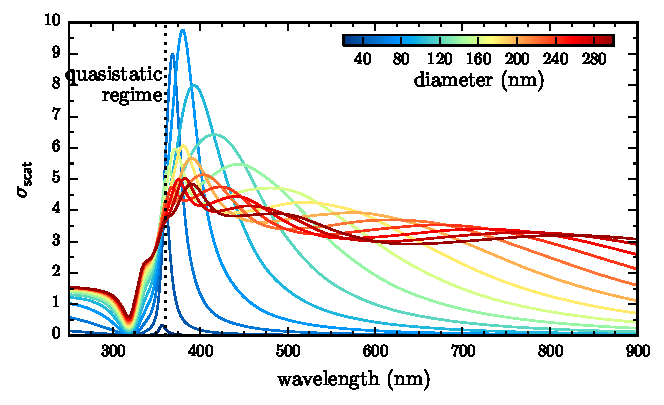
\includegraphics{figures/mie_scattering_ag}
%\caption[Mie scattering {\color{red}efficiencies/cross-sections} for AgNPs of increasing diameter]{\textbf{Mie scattering {\color{red}efficiencies/cross-sections} for AgNPs of increasing diameter.} The \SI{360}{nm} resonance position of the dipolar LSP mode of a AgNP in the quasistatic approximation is indicated by the dotted line. The resonance stays at \SI{360}{nm} until $d>\SI{60}{nm}$ then redshifts. The emergence of higher order modes following a similar behaviour is seen once $d>\SI{100}{nm}$.}
%\label{fig:mie_scattering_ag}
%\end{figure}

\section{Quantum Charge Transport}

One of main discussions of this work is the effect of quantum charge transport on plasmon coupling. Both quantum tunnelling and ballistic transport are qualitatively described in the main text for simplicity. The following section shows the relevant mathematical derivations of the simplest cases of quantum tunnelling and ballistic transport.

\subsection{Quantum Electron Tunnelling}

Electron tunnelling is predicted by the time-independent Schr\"{o}dinger equation for an electron impinging upon a simple rectangular potential barrier, in which,
\begin{equation}
	-\frac{\hbar^2}{2m^*}\frac{d^2\psi(x)}{dx^2} + V(x)\psi(x) = E\psi(x),
\end{equation}
where $m^*$ is the effective electron mass, $V(x)$ is the local potential (either zero or the barrier height $V_0$ depending on the region) and $E$ is the electron energy. A propagating electron incident on the barrier with a wavefunction $\psi = \e^{ikx}$ has an energy given by,
\begin{equation}
	E = \frac{\hbar^2k^2}{2m^*}.
\end{equation}
Inside the barrier the wavefunction decays as $\e^{-\beta x}$ where,
\begin{equation}
	\beta^2 = \frac{2m^*}{\hbar^2}(V_0 - E).
\end{equation}
The transmission probability of the electron passing through the barrier is calculated in the WKB approximation as \cite{griffiths2005introduction},
\begin{align}
	T(E) &= \exp \left\{ -2 \int_0^{d_0} \beta(x) dx \right\}, \\
	&= \exp \left\{ -2 \left[\frac{2m^*}{\hbar^2}(V_0 - E)\right]^{\frac{1}{2}} d_0 \right\}, \label{eq:tunnelling_transmission}
\end{align}
where $d_0$ is the barrier width. Though assuming a simple rectangular barrier, \eqref{eq:tunnelling_transmission} shows the characteristic exponential dependence of electron tunnelling.

\subsection{Ballistic Conduction}

A 1D constriction between two charge reservoirs of length $L$ and width $W$ can be described as either diffusive if $l,l_\phi \ll L,W$, ballistic if $l,l_\phi \gg L,W$, or quasi-ballistic if inbetween, where $l$ and $l_\phi$ are the mean free path and phase coherence length, respectively. Conductance in the diffusive regime is as classically expected, $G=\sigma_{2D}W/L$. In the ballistic regime, however, it inherits quantum properties as is thus given by the Landauer formula,
\begin{equation} G=\frac{2e^2}{h}T(E_F), \end{equation}
where $T(E_F)$ is the transmission coefficient of an electron at the Fermi level. This is derived from the current flowing through a barrier between two biased reservoirs, whereby the Fermi levels are related via $E_{F,L} - E_{F,R} = eV$. The leftwards current through a barrier is given by,
\begin{equation}
	I_L = 2e \int_0^\infty f(E(k), E_{F,L}) v(k) T(k) \frac{dk}{2\pi},
	\label{eq:left_ballistic_current}
\end{equation}
where $f(E, E_F)$ is the Fermi-Dirac function and the wavevector of an electron can be related to its energy via $dE = \hbar v dk$. Converting \eqref{eq:left_ballistic_current} to an energy basis and adding the rightwards current yields,
\begin{equation}
	I_L = \frac{2e}{h} \int_{E_{L}}^\infty \left[ f(E(k), E_{F,L}) - f(E(k), E_{F,R}) \right] T(E) dE.
	\label{eq:ballistic_barrier_current}
\end{equation}
In the small bias limit%
\footnote{Large biases are ignored}
the Fermi-Dirac function is expanded as a Taylor series into,
\begin{equation}
	f(E(k), E_{F,L}) - f(E(k), E_{F,R}) \approx eV \frac{\delta f(E(k), E_F)}{\delta E_F}.
\end{equation}
Substituting this into \eqref{eq:ballistic_barrier_current} yields the integral,
\begin{equation}
	I_L = \frac{2e^2V}{h} \int_{E_{L}}^\infty \left[ -\frac{\delta f}{\delta E} \right] T(E) dE.
\end{equation}
At low temperatures $\delta f/\delta E \rightarrow \delta(E-E_F)$ and the integral evaluates to,
\begin{equation}
	I_L = \frac{2e^2V}{h}T(E_F),
\end{equation}
from which the conductance $G=I/V$ is derived to be,
\begin{equation}
		G = \frac{2e^2}{h}T(E_F).
\end{equation}
With the barrier still in place this corresponds to a tunnelling conductance with $T(E_F)<1$. The point at which the barrier disappears ($E_{barrier} = E_F$) gives rise to $T(E) = 1$ and opens up a single quantised conductance channel. Adding additional $n$ sub-bands into the constriction continues to increase the conductance by its quantum, $2e^2/h$, and thus the conductance of a 1D \emph{conductive} junction can be expressed as,
\begin{equation}
	G = \frac{2e^2}{h}n.
\end{equation}

\FloatBarrier
\chapter{Supplementary Experimental Details}

\section{Supplementary Optical Details}

\begin{figure}[bt]
\centering
\fontsize{10pt}{1em}\selectfont
\def\svgwidth{0.9\textwidth}
\subimport{./figures/}{reimaging_concept.pdf_tex}
\caption[Concept of reimaging for beam alignment]{\textbf{Concept of reimaging for beam alignment.} (a) Adjusting the angle of the beam in a focal plane does not change the position of the focus in the image (front focal) plane but changes the position in the Fourier (back focal) plane. (b) Adjusting the angle of the beam in a Fourier plane translates the position of the beam in the image plane without changing its angular components.}
\label{fig:reimaging_concept}
\end{figure}

Features, design justifications and optical theory not essential to the main text are detailed here, including notes on reimaging, choice of objectives and polarisation optimisation. The concept of reimaging, and its effect on beam alignment, is shown in \autoref{fig:reimaging_concept}. The ray diagrams show that the beam position in the focus can be adjusted by changing the angle of a mirror placed in the Fourier plane (in the case of the microscope the mirror directly after the DF stop). The shape of the beam, dictated by its angular distribution in Fourier space, is controlled by tilting a mirror in a focal plane (the mirror in the focus of the reimaging arm). The two mirrors provide independent control over the two main beam properties.

\begin{figure}[bt]%{O}{9cm}
\vspace{-10pt}
\centering
\fcapside[\FBwidth]
{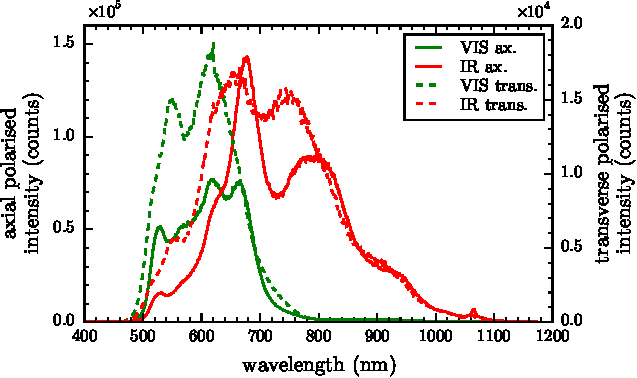
\includegraphics{figures/objective_comparison}}
{\caption[Spectral comparison between VIS and IR objectives]{\textbf{Spectral comparison between VIS and IR objectives.} The VIS objective is an Olympus $100\times$ 0.9\,NA MPlan BD dark-field objective whereas the IR objective is an Olympus $100\times$ 0.8\,NA MPlan bright-field objective.}
\label{fig:objective_comparison}}
\vspace{-5pt}
\end{figure}

The choice of objective was determined by the overall range over which a reference spectrum from a Ag mirror is valid. Two long working distance objectives suitable for single nanostructure spectroscopy were characterised for use in the microscope: a VIS and an IR objective. The raw reflectance spectrum of the supercontinuum laser measured using each objective is shown in \autoref{fig:objective_comparison}. The short wavelength cut-off at \SI{480}{nm} is due to the supercontinuum laser. The VIS objective clearly outperforms the IR objective below \SI{625}{nm}, though both objective counts are large enough to maintain a good reference signal. Overall, references using the VIS objective only extend marginally more below \SI{500}{nm}. However, the \SI{700}{nm} cut-off of the VIS objective means that it is not suitable for spectra in the NIR with referencing only valid up until \SI{900}{nm} whereas the IR objective extends to \SI{1100}{nm}. The gain in spectral range means that the IR objective is chosen despite its lack of dark-field illumination for imaging.

\begin{wrapfigure}{O}{9cm}
\vspace{-10pt}
\centering
%\fcapside[\FBwidth]
{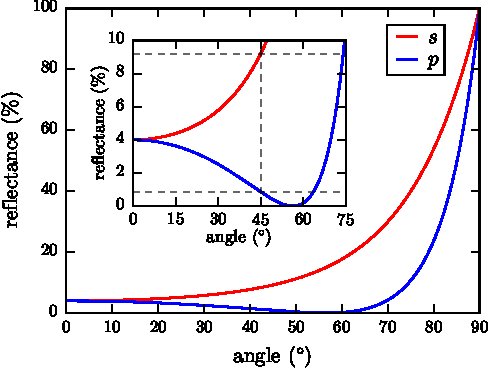
\includegraphics{figures/fresnel_coefficients}}
{\caption[Reflectance as a function of angle of incidence for glass-air interface]{\textbf{Reflectance as a function of angle of incidence for glass-air interface.} Reflective is calculated from the fresnel coefficients. The refractive index of glass is assumed to be $n=1.5$. The inset shows a zoomed segment at low reflectances.}
\label{fig:fresnel}}
\vspace{-5pt}
\end{wrapfigure}

Consideration was given when designing the optical layout to account for intensity differences in each linear polarisation. Reflection and transmission of an EM wave incident on an interface between two refractive media at an angle is governed by the Fresnel equations \cite{grant2013electromagnetism}. As shown in \autoref{fig:fresnel}, there is a large difference in reflectance between linear polarisations at higher angles of incidence. The microscope is designed such that the $s$-polarisation corresponds to light polarised along the tip axis, maximising its transmission to the spectrometers. Leakage of the $s$-polarisation into the weaker $p$-polarisation signal at the polarising beamsplitter limits current polarisation resolved measurements.

%\subsection{Optical Characterisation}

%\begin{figure}[bt]
%\centering
%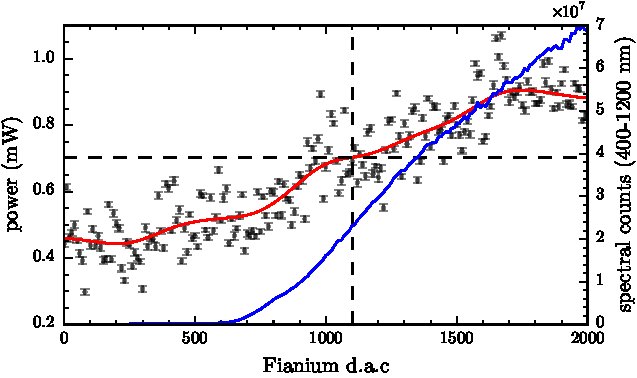
\includegraphics{figures/fianium_power}
%\caption
%[Fianium power incident on the back aperture of the objective as a function of driving current.]
%{\textbf{Fianium power incident on the back aperture of the objective as a function of driving current.} The beam diameter is restricted to the size of the back aperture to accurately measure the power throughput without measuring extra power not transmitted to the sample plane. Error bars represent the precision (standard error) of 1000 repeat measurements at each power, hence they are small, however the large distribution of points shows that the power meter is only accurate to \SI{1}{mW}.}
%\label{fig:fianium_power}
%\end{figure}

%The measured broadband power incident on the back aperture of the objective (removing the contribution from over-filling of the back aperture using an iris) is shown in \autoref{fig:fianium_power}. The power is measured using a thermopile bolometer (Coherent Powermax) with simultaneous measurements of the spectral counts of the $s$-polarised signal component summed between 400--\SI{1200}{nm}. The supercontinuum laser is driven with a d.a.c. of 1100 in most experiments. Under these conditions, less than \SI{1}{mW} is used to illuminate samples, enough that reflection from a reference substrate just under saturates the spectrometer counts. Assuming a spot size on \orderof{\SI{1}{\micro\metre}} means a focal intensity of \SI{e5}{\watt\per\centi\metre\squared}. Sub-mW powers are sufficient to maintain good signals without risking damage to nanoscale samples.

\section{Supplementary Electronics}

\begin{figure}[b]
\centering
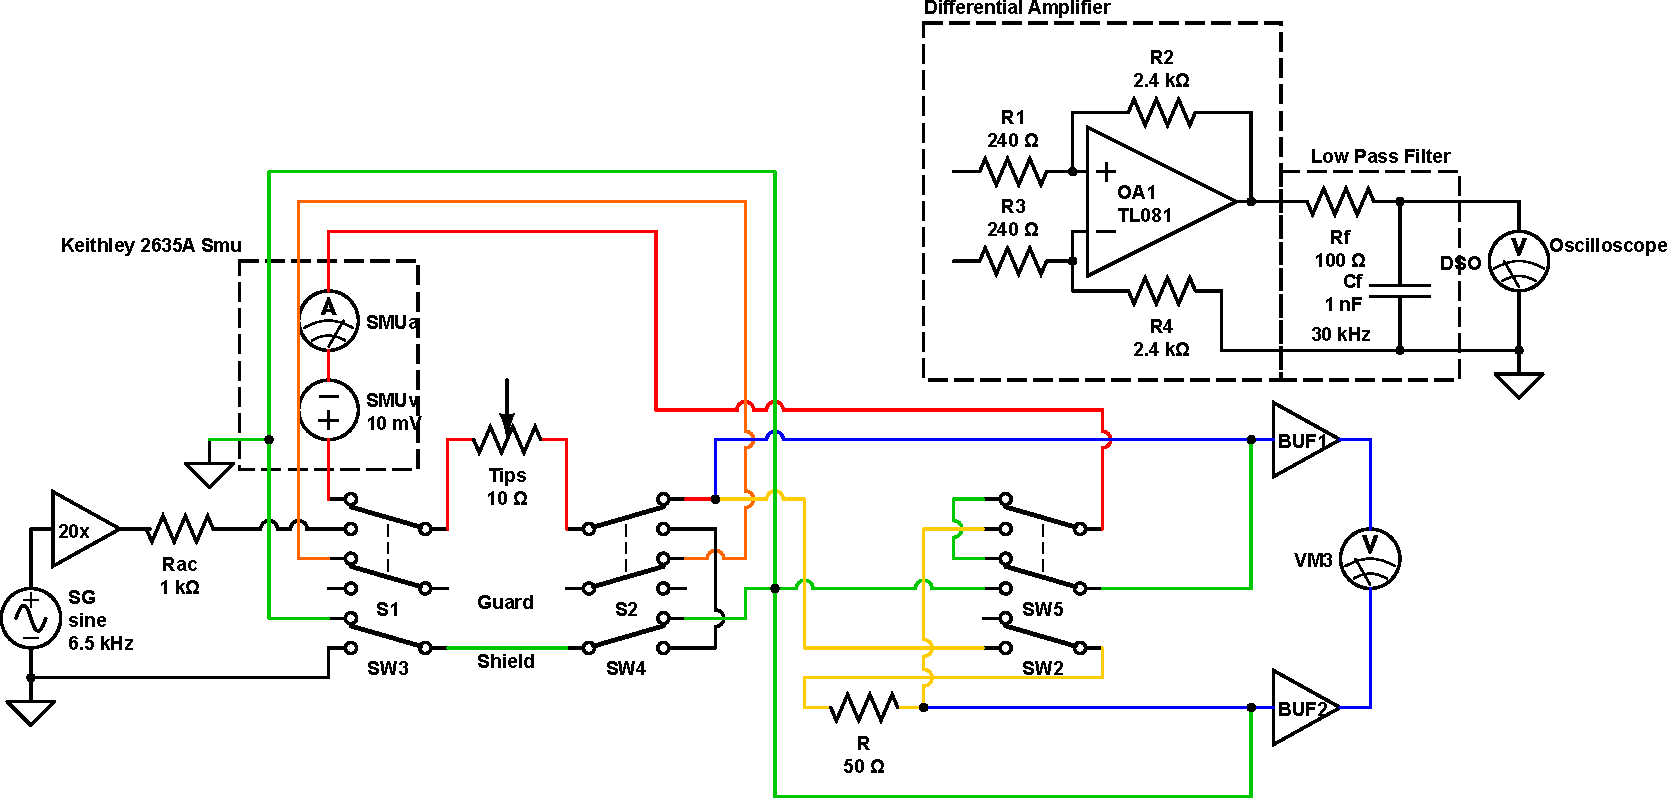
\includegraphics[width=0.9\textwidth]{figures/tip_experiment_circuit_design}
\caption[Schematic of the electrical measurement circuit.]{\textbf{Schematic of the electrical measurement circuit.} The central routing box allows switching between a.c.\ and d.c.\ circuits and low-and high-bandwidth d.c.\ measurements. The a.c.\ circuit is used to align two AFM probes together while the d.c.\ circuit is used to measure spatially dependent signals from the gap between two AFM probes.}
\label{fig:circuit_design}
\end{figure}

The schematic circuitry of the microscope electronics is shown in \figref{fig:circuit_design}, corresponding to the simpler block diagram shown in the main text.

\section{Software Lock-In Derivation}

To lock into only the signal component at the reference frequency $\omega_r$ a reference wave needs to be computed. The first step in the lock-in process is to mathematically construct a single frequency waveform at the correct harmonic using the supplied reference signal. The reference signal is typically of the form $A\sin(\omega_{rs} t + \phi_r)$, but the algorithm will also work with any periodic function since it triggers off a rising position edge.
When $\sin(\theta)=0$ and the gradient is positive ($\cos(\theta)=1$) $\theta=2n\pi$. Hence the rising edge trigger points $t_i$ occur at,
\begin{equation} \theta = \omega_{rs} t_i + \phi_r = 2n\pi. \end{equation}
Trigger times are fitted against the number of triggers (number of periods) since the start of the signal using,
\begin{equation}
t_i = \frac{1}{\omega_{rs}}(2n\pi - \phi_r) = \frac{2\pi}{\omega_{rs}}n - \frac{\phi_r}{\omega_{rs}}.
\end{equation}
A complex reference wave of the form $e^{ih(\omega_{rs} t + \phi_r)}$, where $h$ is the harmonic of the reference frequency $\omega_{rs}$ required to lock into the frequency $\omega_r$, is constructed from the $t_i=mn+c$ fit using,
\begin{align}
\omega_{rs} &= \frac{2\pi}{m}, \\
\phi_r &= \frac{mc}{2\pi}.
\end{align}
The frequency component of the signal at $\omega_r=h\omega_{rs}$ can be extracted using Fourier analysis,
\begin{equation}
Z_s(\omega_r) = \frac{2}{t} \int_0^t{Z_s(t) e^{-ih(\omega_{rs} t + \phi_r)} dt}.
\end{equation}
Discretising this not a programmable form results in,
\begin{equation}
Z_s(\omega_r) = \frac{2}{n} \sum_0^n{Z_s(t_n) e^{-ih(\omega_{rs} t_n + \phi_r)}}
\end{equation}
where $\real{Z_s(\omega_r)}$ and $\imag{Z_s(\omega_r)}$ are the $x$ and $y$ of the signal component at $\omega_r$, respectively. Polar coordinates of amplitude and phase are retrieved using the coordinate transforms,
\begin{align}
r = \sqrt{x^2 + y^2}, \\
\phi = \tan^{-1}(y/x).
\end{align}

\section{Capacitive Alignment Model Derivation}

The equation of motion for the dual-tip system is derived in the main text as,
\begin{equation}
	m_1 \frac{d^2z_1}{dt^2} + \beta_{01}^z \frac{dz_1}{dt} + k_{01}^z (z_1-d_0) = \left( \frac{-\varepsilon_0 A_{ov} V_0^2}{4z_1^2}\right)\left[1+\cos(\omega_pt)\right].
\label{eq:final_eom_app}
\end{equation}
Expressing \eqref{eq:final_eom_app} in terms of $z_r = z - d_0$ yields,
\begin{equation}
	m_1 \frac{d^2z_r}{dt^2} + \beta_{01}^z \frac{dz_r}{dt} + k_{01}^zz_r = \left( \frac{-\varepsilon_0 A_{ov} V_0^2}{4(z_r+d_0)^2}\right)\left[1+\cos(\omega_pt)\right],
\label{eq:final_rel_eom_app}
\end{equation}
and enables further simplification via approximation. Assuming that $z_r \ll d_0$ the right hand side of \eqref{eq:final_rel_eom_app} can be taken to first order using a Taylor series,%
\footnote{$F(z_r) = F(0) + \left.\frac{dF(z_r)}{dz_r}\right\rvert_0 z_r = \left(\frac{-\varepsilon_0 A_{ov} V_0^2}{4}\right) [1+\cos(\omega_pt)] \left(\frac{1}{d_0^2} - \frac{2z_r}{d_0^3 }\right)$}
%
\begin{equation}
m_1 \frac{d^2z_r}{dt^2} + \beta_{01}^z \frac{dz_r}{dt} + k_{e1}^zz_r \simeq \left(\frac{-\varepsilon_0 A_{ov} V_0^2}{4d_0^2}\right) \left[1+\cos(\omega_pt)\right],
\label{eq:first_order_eom_app}
\end{equation}
%
where,
%
\begin{equation}
k_{e1}^z = k_{01}^z - \left(\frac{\varepsilon_0 A_{ov} V_0^2}{2d_0^3}\right) \left[1+\cos(\omega_pt)\right].
\end{equation}
This effective spring constant $k_{e1}^z$ does not cause parametric mixing as it oscillates at $\omega_p$ therefore its effect can be averaged out over time resulting in $\langle k_{e1}^{z} \rangle = k_{01}^z - {\varepsilon_0 A_{ov} V_0^2}/{2d_0^3}$. The EoM is then once again approximated to,
\begin{equation}
m_1 \frac{d^2z_r}{dt^2} + \beta_{01}^z \frac{dz_r}{dt} + \langle k_{e1}^{z} \rangle z_r \simeq \left(\frac{-\varepsilon_0 A_{ov} V_0^2}{4d_0^2}\right) \left[1+\cos(\omega_pt)\right],
\end{equation}

Defining the constant $q$ as,
\begin{equation} q = \left(\frac{-\varepsilon_0 A_{ov} V_0^2}{4d_0^3}\right), \end{equation}
the effective spring constant can be expressed as,
\begin{align}
k_{e1}^z &= k_{01}^z + 2q \left[1+\cos(\omega_pt)\right],\\
\langle k_{e1}^{z} \rangle &= k_{01}^z + 2q,
\end{align}
and the EOM can be again rewritten in the form,
\begin{equation}
m_1\ddot{z_r} + \beta_{01}^z\dot{z_r} + \left[\langle k_{e1}^z\rangle + 2q\cos(\omega_pt)\right]z_r - q\left[1+\cos(\omega_pt)\right]d_0 \simeq 0,
\label{eq:first_order_simple_eom_app}
\end{equation}
Equation \eqref{eq:first_order_simple_eom_app} is of the form of the driven damped Mathieu equation,
\begin{equation} \ddot{z} + 2\kappa\dot{z} + [a - 2q\cos(2t)]z = F(t), \end{equation}
and has solutions in the limit of small oscillations of \cite{savage2012thesis},
\begin{equation}
z_1 \approx d_0 - \left|z_{1}^{off}\right| - z_{m1}\cos(\omega_pt+\varphi_1)
\label{eq:tip_oscillation_app}
\end{equation}
where
\begin{subequations}
\begin{align}
z_1^{off} &\approx %
\frac{ \varepsilon_0 A_{ov} V_0^2 }{ 4d_0^2 \langle k_{e1}^z \rangle }, \label{eq:tip_amp_app}\\
%
z_{m1} &\approx %
\frac{ \varepsilon_0 A_{ov} V_0^2 }%
{ 4d_0^2 \sqrt{ (\langle k_{e1}^z \rangle - m_1\omega_p^2)^2 + (\beta_{01}^z\omega_p)^2  } }, \\
%
\varphi_1 &\approx \tan^{-1}\left(\frac{\beta_{01}^{z}\omega_{p}}{\langle k_{e1}^{z} \rangle -m_{1}\omega_{p}^{2}}\right). \label{eq:tip_phase_app}
\end{align}
\end{subequations}

\subimport{./}{fast_spectroscopy}

\begin{singlespace}
\printbibliography[category=appendices, resetnumbers=true, title={Supplementary Bibliography}]
\end{singlespace}

\end{document}